\chapter*{Traversée de Chiloe\markboth{Traversée de Chiloe}{}}
\section*{22 février 2015}
6 jours pour traverser l´île de Chiloe en vélo du nord au sud. \newline
 Je commence à descendre par la route principale ce qui permet d´avancer bien car la route est goudronnée et avec des montées raisonnables. \newline
 \newline
\centerline{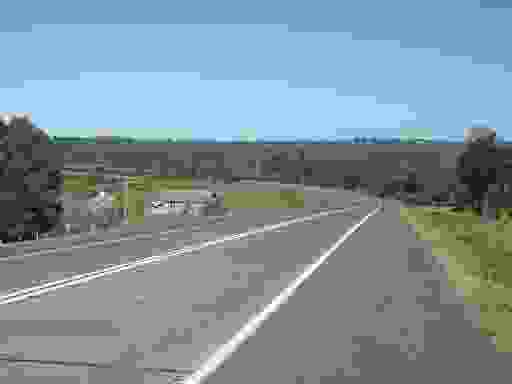
\includegraphics[width=\mywidth]{../wp-content/uploads/2015/02/P2132099.jpg} } 
 \newline
 Suite en direction de la côte à l´est, on apercoit quelques sommets de la cordillère des Andes au loin. \newline
 \newline
\centerline{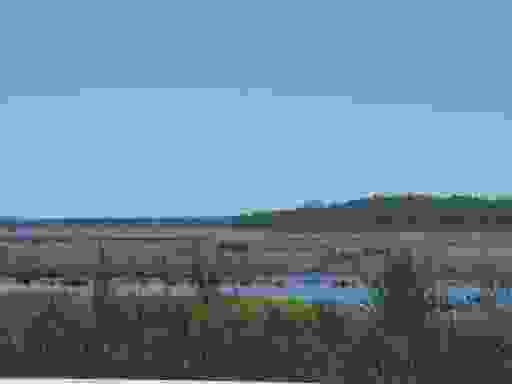
\includegraphics[width=\mywidth]{../wp-content/uploads/2015/02/P2132098.jpg} } 
 \newline
 \newline
\centerline{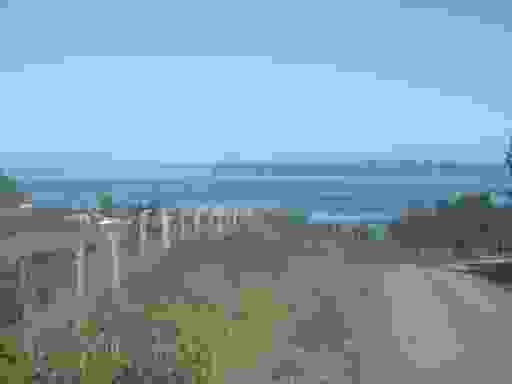
\includegraphics[width=\mywidth]{../wp-content/uploads/2015/02/P2142124.jpg} } 
 \newline
 Visite d´un petit îlot \newline
 \newline
\centerline{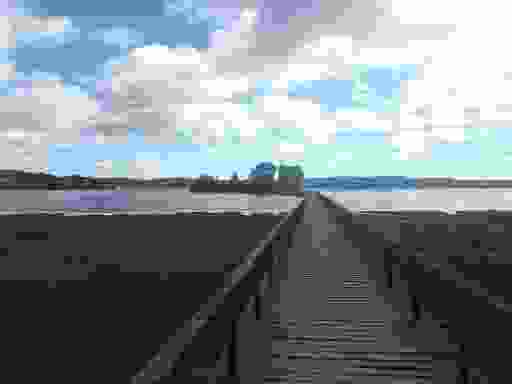
\includegraphics[width=\mywidth]{../wp-content/uploads/2015/02/P2142106.jpg} } 
 \newline
 \newline
\centerline{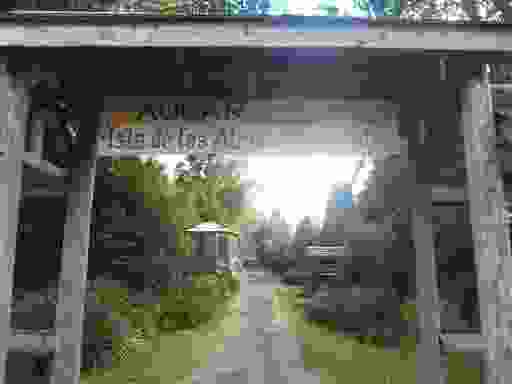
\includegraphics[width=\mywidth]{../wp-content/uploads/2015/02/P2142108.jpg} } 
 \newline
 \newline
\centerline{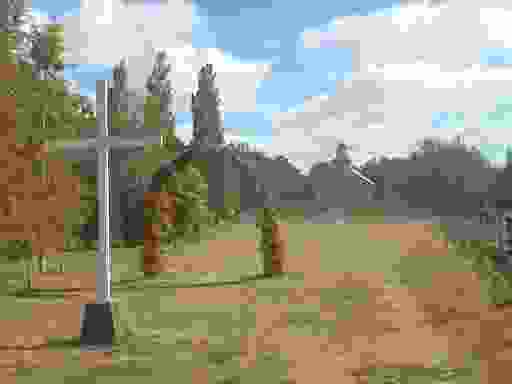
\includegraphics[width=\mywidth]{../wp-content/uploads/2015/02/P2142109.jpg} } 
 \newline
\centerline{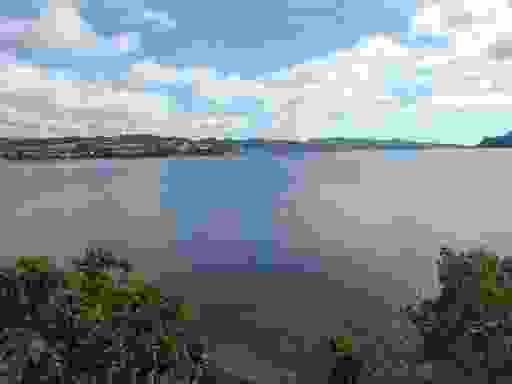
\includegraphics[width=\mywidth]{../wp-content/uploads/2015/02/P2142110.jpg} } 
 \newline
 Passage par une partie de la route des églises de Chiloe, plusieurs d´entres elles sont au patrimoine de l´Unesco. \newline
 Eglise de Colo, 3km de piste aller retour super raide pour y arriver, ca se mérite ! \newline
 \newline
\centerline{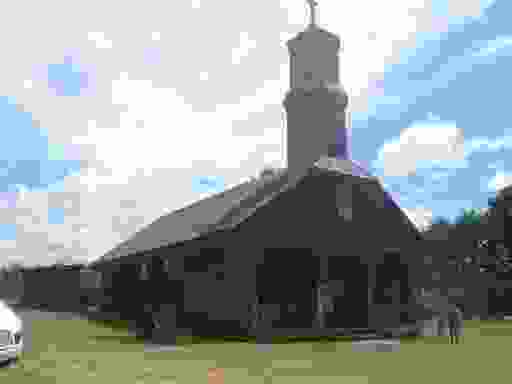
\includegraphics[width=\mywidth]{../wp-content/uploads/2015/02/P2142113.jpg} } 
 \newline
 Eglise de Castro \newline
 \newline
\centerline{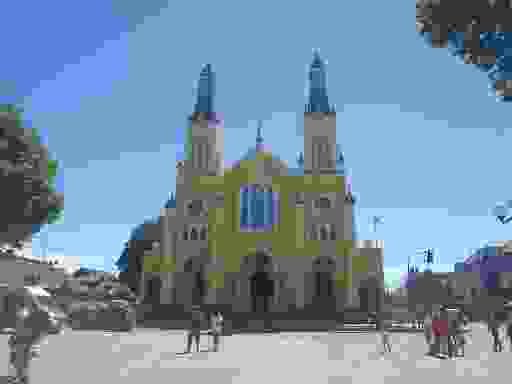
\includegraphics[width=\mywidth]{../wp-content/uploads/2015/02/P2152142.jpg} } 
 \newline
 Eglise de Nercon \newline
 \newline
\centerline{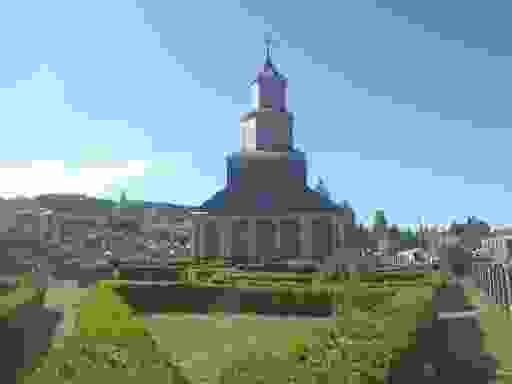
\includegraphics[width=\mywidth]{../wp-content/uploads/2015/02/P2152150.jpg} } 
 \newline
 Après je les ai pas toutes vues, il y en a une vingtaine au total. \newline
 Passage par une cascade sympathique \newline
 \newline
\centerline{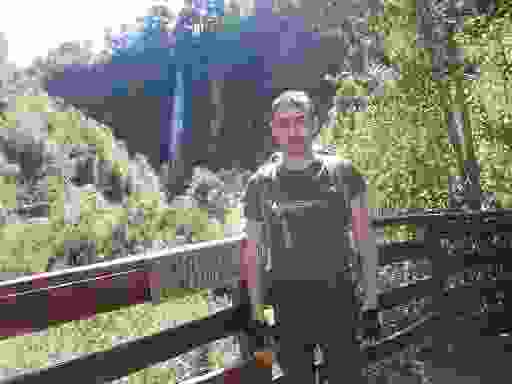
\includegraphics[width=\mywidth]{../wp-content/uploads/2015/02/P2142119.jpg} } 
 \newline
 Juste avant d´arriver à Castro, la capitale de l´île je me fais rattraper par Jérémy que j´avais croisé à Ancud. Il voyage en vélo depuis 2 ans et demi, il a déjà parcouru la route entre terre de feu et le Canada. Il est revenu dans le sud pour faire quelques endroits qu´il ne connait pas encore ! \newline
 \newline
\centerline{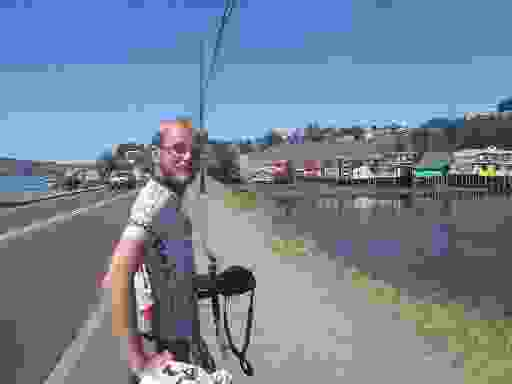
\includegraphics[width=\mywidth]{../wp-content/uploads/2015/02/P2152135.jpg} } 
 \newline
 Puisque nous allons tous les 2 vers le sud de l´île, nous continuons la route ensemble. \newline
 Castro et ses maisons sur pilotis \newline
 \newline
\centerline{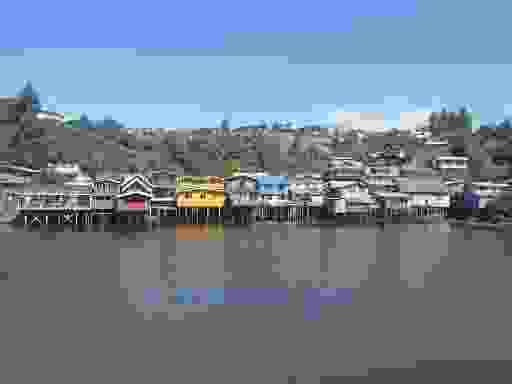
\includegraphics[width=\mywidth]{../wp-content/uploads/2015/02/P2152133.jpg} } 
 \newline
 \newline
\centerline{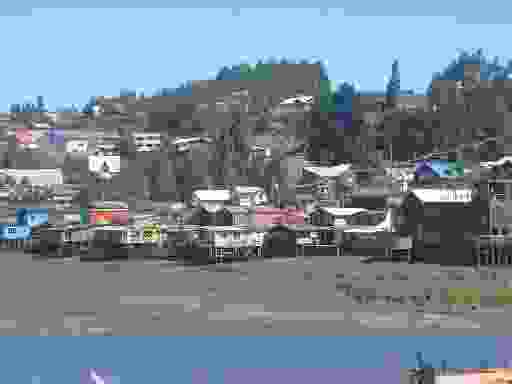
\includegraphics[width=\mywidth]{../wp-content/uploads/2015/02/P2152146.jpg} } 
 \newline
 Je fais bien du vélo ici \newline
 \newline
\centerline{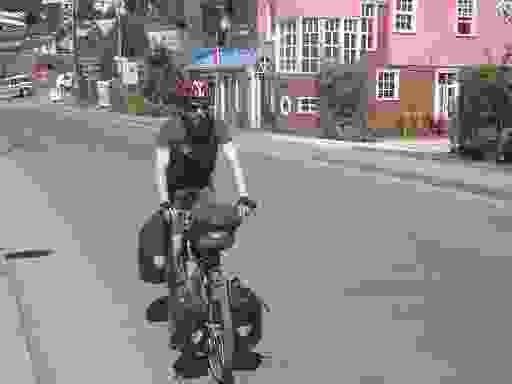
\includegraphics[width=\mywidth]{../wp-content/uploads/2015/02/P2152141.jpg} } 
 \newline
 Petite fête locale avec de la musique et des spécialités culinaires \newline
 \newline
\centerline{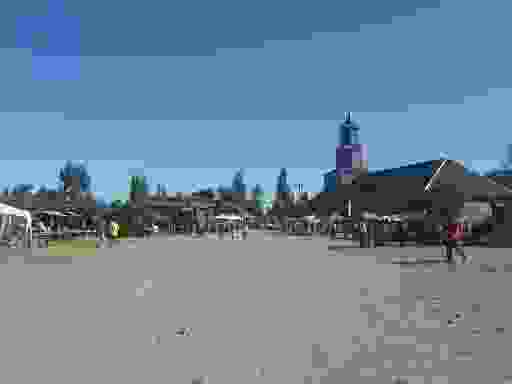
\includegraphics[width=\mywidth]{../wp-content/uploads/2015/02/P2152151.jpg} } 
 \newline
 Après Castro, nous repartons vers la côte Pacifique et le parc national de Chiloe. \newline
 La route longe un beau lac, l´occasion de se rafraichir \newline
 \newline
\centerline{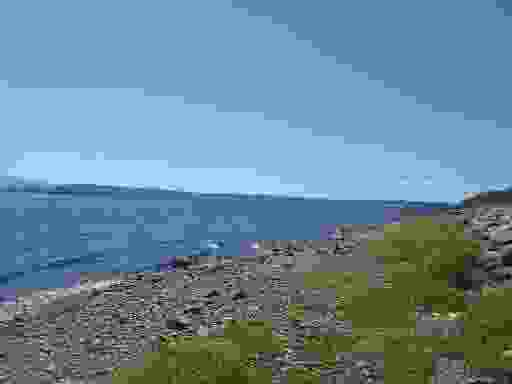
\includegraphics[width=\mywidth]{../wp-content/uploads/2015/02/P2162156.jpg} } 
 \newline
 \newline
\centerline{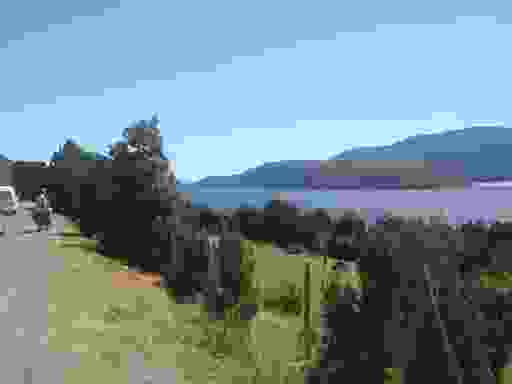
\includegraphics[width=\mywidth]{../wp-content/uploads/2015/02/P2162158.jpg} } 
 \newline
 \newline
\centerline{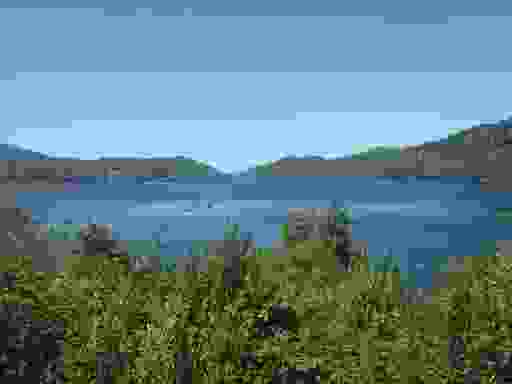
\includegraphics[width=\mywidth]{../wp-content/uploads/2015/02/P2162161.jpg} } 
 \newline
 Plage immense au bord du pacifique \newline
 \newline
\centerline{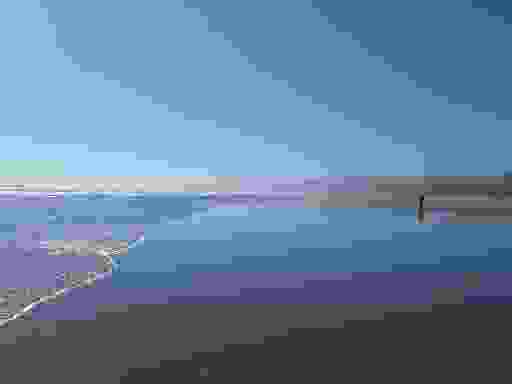
\includegraphics[width=\mywidth]{../wp-content/uploads/2015/02/P2162164.jpg} } 
 \newline
 Bivouac à quelques mètres de la plage \newline
 \newline
\centerline{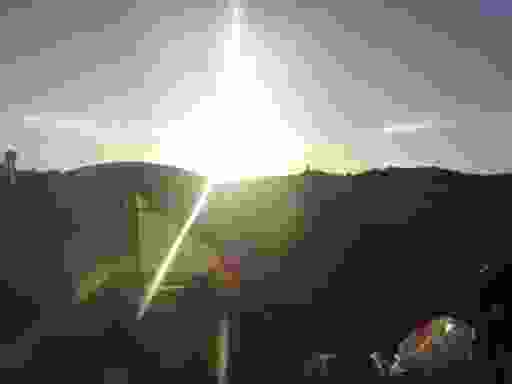
\includegraphics[width=\mywidth]{../wp-content/uploads/2015/02/P2172173.jpg} } 
 \newline
 \newline
\centerline{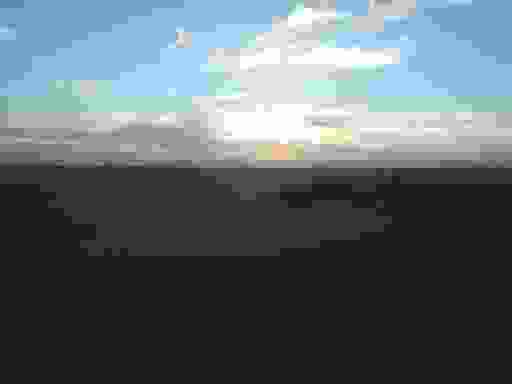
\includegraphics[width=\mywidth]{../wp-content/uploads/2015/02/P2172175.jpg} } 
 \newline
 \newline
\centerline{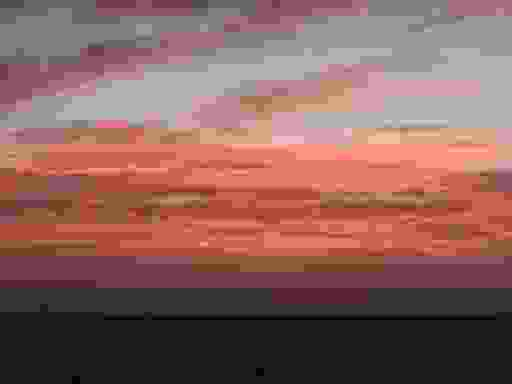
\includegraphics[width=\mywidth]{../wp-content/uploads/2015/02/P2172180.jpg} } 
 \newline
 Balade dans le parc national qui contient des forêts très denses et à la végétation particulière \newline
 \newline
\centerline{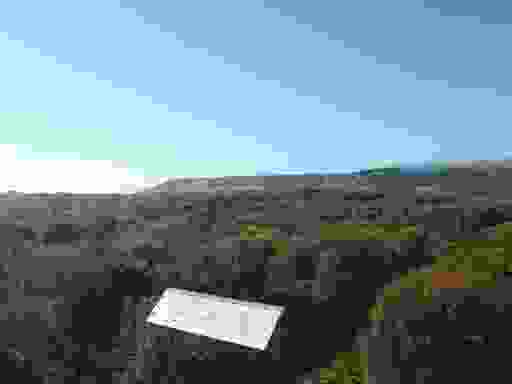
\includegraphics[width=\mywidth]{../wp-content/uploads/2015/02/P2162167.jpg} } 
 \newline
 \newline
\centerline{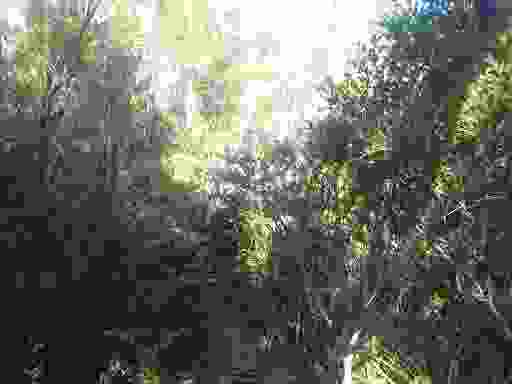
\includegraphics[width=\mywidth]{../wp-content/uploads/2015/02/P2162169.jpg} } 
 \newline
 Dernier bivouac avant de quitter Chiloe \newline
 \newline
\centerline{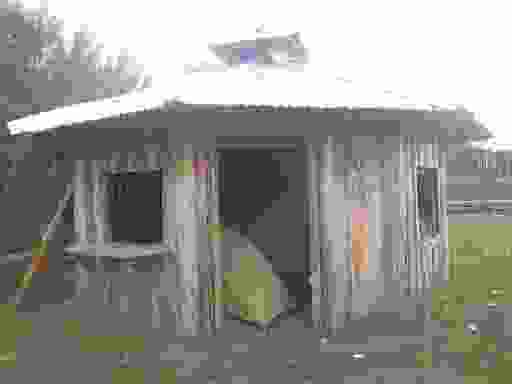
\includegraphics[width=\mywidth]{../wp-content/uploads/2015/02/P2172189.jpg} } 
 \newline
 Et encore quelques spécialités locales sur la route \newline
 Les empanadas, il y en a partout avec différentes garnitures, viande, fromage, légumes… \newline
 \newline
\centerline{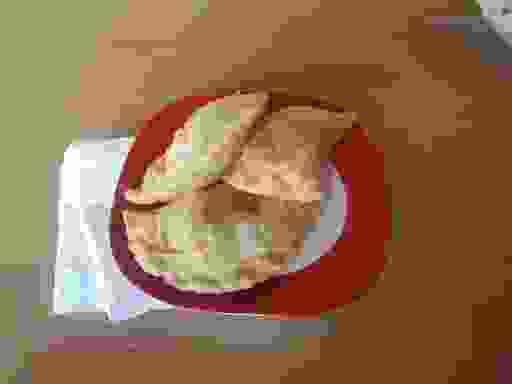
\includegraphics[width=\mywidth]{../wp-content/uploads/2015/02/P2142116.jpg} } 
 \newline
 Le Curanto, typique de Chiloe, coquillages, saucisse, porc, pomme de terre et fèves, le tout cuit dans des pierres chaudes. \newline
 \newline
\centerline{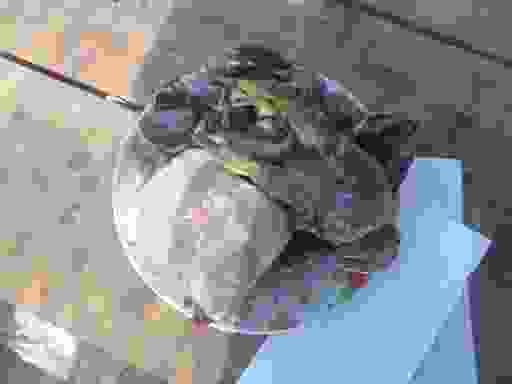
\includegraphics[width=\mywidth]{../wp-content/uploads/2015/02/P2152152.jpg} } 
 \newline
 Le Mote con Huesilla, boisson sucrée avec une pêche et des grains de blé au fond \newline
 \newline
\centerline{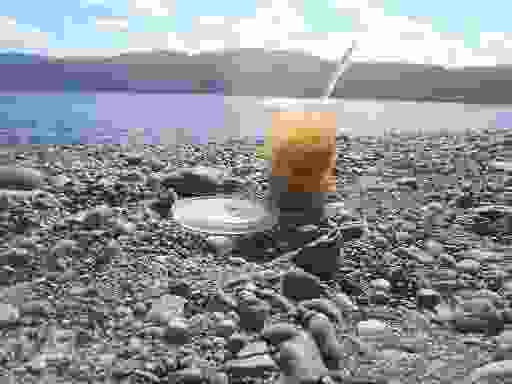
\includegraphics[width=\mywidth]{../wp-content/uploads/2015/02/P2172183.jpg} } 
 \newline

\newpage
 
